\chapter{Generación de Melodías con \textit{Machine Learning}}
\label{cap:generacionMusical}

En este capítulo se explicará cómo hemos generado melodías. Se van a explorar distintas formas de generación de melodías, entre ellas 2 modelos entrenados por nosotros y un modelo ya existente de Magenta. 

\section{Cómo representamos la música}
Para poder trabajar con las melodías, necesitamos alguna forma de representación interna para tratar las notas en los diferentes modelos. A continuación se detallan las representaciones utilizadas.

\label{sec:como-generamos-melodias}
    \subsection{Representación \textit{"pitch\_duration"}}
    \label{sub:representacion-pitch_duracion}
    Esta representación simplifica al máximo la información crucial de una nota, es utilizada tanto por las Cadenas de Markov (explicadas en Sección \ref{sec:Markov-chain}), como por las Redes Neuronales Recurrentes (explicadas en Sección \ref{sec:RNR}).

    La duración suele venir dada en steps, ya que nos proporcionan una unidad entera que es independiente del tiempo absoluto.

    Las notas se supone que se encuentran seguidas una de otra y no pueden sonar varias a la vez, por lo que no son necesarios atributos como el tiempo de inicio o fin de cada nota.

    El silencio viene codificado como una nota de pitch 0.

    Por ejemplo, si quisiéramos codificar un Do de la cuarta octava (C4 en inglés) que dura 2 tiempos se codificaría como "60\_2", siendo 60 el pitch MIDI de la nota C4 (consultar \cite{MIDIPitch} para más información sobre el pitch MIDI).

    \subsection{Magenta NoteSequence}
    \label{subsec:note-seq}
    
    En las partes de generación de melodías que utilizan machine learning empleamos el estándar definido por Magenta llamada NoteSequence: \cite{note-seq}. 

    Este estándar nos proporciona una forma cómoda y rápida de interactuar con la API de Magenta (explicada en Sección \ref{sec:magenta}), así como de poder leer y convertir a MIDI fácilmente.

    Existe un paquete de pip para utilizar NoteSequence en Python llamado \textit{note-seq}.

    En el módulo propio \textit{noteseqConverter} se definen una serie de funciones para poder convertir de NoteSequence al formato simplificado \textit{"pitch\_duración"} y a json, así como funciones para guardar y cargar archivos MIDI.

\section{Dataset utilizado y procesamiento de datos}
\label{sec:dataset}
Para poder utilizar algoritmos de machine learning lo primero es tener un dataset con una gran cantidad de datos y procesarlo adecuadamente.

A la hora de buscar el dataset es importante buscar uno adecuado para poder generar melodías básicas que podamos posteriormente armonizar y crear variaciones de esta.

Magenta posee una gran cantidad de datasets que se utilizaron para el entrenamiento de sus modelos. Dichos datasets se pueden consultar en \cite{MagentaDatasets}.

El dataset elegido ha sido el \textit{Bach Doodle Dataset} de Magenta\footnote{\url{https://magenta.tensorflow.org/datasets/bach-doodle}}.

Este dataset consiste en una serie archivos JSON con melodías que componían los usuarios del Bach Doodle (\cite{BachDoodlePaper}). Contiene más de 6 años de música de usuarios y sus melodías están en formato NoteSequence (para más información ver Sección \ref{subsec:note-seq}).

Al utilizar un dataset con melodías sencillas podemos entrenar de forma más simple y directa nuestros modelos. Pero para poder utilizar el dataset tenemos que procesar algunos aspectos de este:

\begin{itemize}
\item Lo primero es filtrar las melodías. Existe un campo en cada entrada del dataset llamado \textit{"feedback"}, que representa el feedback de usuarios con 0 (malo), 1 (neutral) o 2 (positivo). Ya que tenemos una gran cantidad de melodías, podemos descartar todas las melodías que no tengan un feedback de 2.

\item Para poder realizar ajustes posteriormente a la melodía es conveniente que se encuentre en una escala determinada. El dataset incluye un campo llamado \textit{"key\_sig"}, el cual indica la nota fundamental de la escala. Por simplicidad descartamos todas las melodías que no se encuentren en Do Mayor (C Major en inglés). Además, limitamos las notas a 2 octavas realizando trasposiciones de estas.

\item Finalmente, es vital normalizar el tempo de las canciones, por lo que convertimos todas las melodías a 120bpm. Para esto basta con convertir adecuadamente los steps de las melodías del dataset, ya que existe un campo llamado \textit{"tempos"} en la propia NoteSequence de la melodía.

\end{itemize}

Una vez realizados estos ajustes, podemos guardar el dataset procesado como CSV con los atributos
\begin{center}
    \textit{pitch}, \textit{start}, \textit{end}, \textit{duration}, \textit{next\_note\_pitch}, \textit{next\_note\_start}, \textit{next\_note\_duration}.
\end{center}
Con estos parámetros podemos implementar distintos modelos de machine learning utilizando unos parámetros u otros dependiendo de las necesidades del modelo.

\section{Cadenas de Markov}
\label{sec:Markov-chain}

    Las cadenas de Markov son un modelo estocástico que describe una secuencia de eventos en la que la probabilidad de cada evento es dependiente únicamente del estado anterior.

    Por lo tanto, el modelo de Markov no tiene memoria (sin entrar a modelos más complejos).

    Simplificando, podemos pensar en las cadenas de Markov como una máquina de estados en la que cada estado está conectado a todos los demás y las probabilidades de pasar a cada estado desde uno cualquiera suman 1.

    Las cadenas de Markov son comúnmente representadas gráficamente mediante un grafo dirigido tal y como se muestra en la Figura \ref{fig:sampleChain1}.

    \begin{figure}[h]
    \centering
    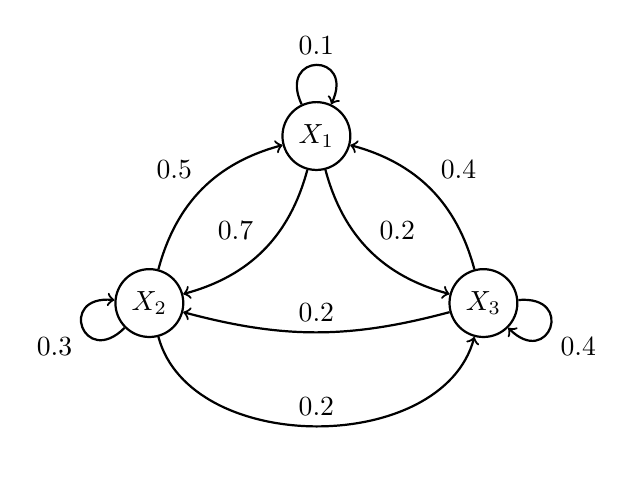
\begin{tikzpicture}[node distance={30mm}, thick, main/.style = {draw, circle}] 
    \node[main] (1) {$X_1$}; 
    \node[main] (2) [below left of=1] {$X_2$}; 
    \node[main] (3) [below right of=1] {$X_3$};
    \draw[->] (1) to [out=115,in=65,looseness=5] node[midway, above, pos=0.5] {0.1} (1);
    \draw[->] (1) to [out=-105,in=15,looseness=1] node[midway, above left, pos=0.5] {0.7} (2);
    \draw[->] (1) to [out=-75,in=165,looseness=1] node[midway, above right, pos=0.5] {0.2} (3);
    \draw[->] (2) to [out=75,in=195,looseness=1] node[midway, above left, pos=0.5] {0.5} (1);
    \draw[->] (2) to [out=225,in=175,looseness=5] node[midway, below left, pos=0.5] {0.3} (2);
    \draw[->] (2) to [out=285,in=255,looseness=1] node[midway, above, pos=0.5] {0.2} (3);
    \draw[->] (3) to [out=105,in=-15,looseness=1] node[midway, above right, pos=0.5] {0.4} (1);
    \draw[->] (3) to [out=195,in=-15,looseness=1] node[midway, above, pos=0.5] {0.2} (2);
    \draw[->] (3) to [out=5,in=-45,looseness=5] node[midway, below right, pos=0.5] {0.4} (3);
    \label{fig:sampleChain1}
    \end{tikzpicture}
    \caption{Ejemplo de una cadena de Markov} 
    \label{fig:sampleChain1}
    \end{figure}
    
    Internamente, las cadenas de Markov se suelen representar con matrices de transición, tales como la de la tabla \ref{tab:sampleChainMatrix}

    \begin{table}[h]
	\centering
	\begin{tabular}{c|c|c|c}
		\textbf{} & \textbf{$X_1$} & \textbf{$X_2$} & \textbf{$X_3$}\\
		\hline
		\textbf{$X_1$} & 0.1 & 0.7 & 0.2\\
		\hline
		\textbf{$X_2$} & 0.5 & 0.3 & 0.2\\
		\hline
		\textbf{$X_3$} & 0.4 & 0.2 & 0.4\\
	\end{tabular}
	\caption{Ejemplo de una matriz de transición}
	\label{tab:sampleChainMatrix}
    \end{table}
    
    \subsection{Entrenamiento de las Cadenas de Markov}
    \label{subsec:entrenamientoCadenasMarkov}
    Una ventaja de las cadenas de Markov es su fácil entrenamiento. Una vez tenemos nuestro dataset limpio y normalizado (como se explica en Sección \ref{sec:dataset}) podemos recorrerlo para construir la matriz de transición.

    En nuestro caso, cargamos todas las secuencias de notas del dataset, descartamos las notas que no tienen otra a continuación (serían las que se encuentran al final de la melodía) y rellenamos una tabla de ocurrencias. Dicha tabla indica el número de veces que una nota aparece después de otra en las melodías.

    Por ejemplo, si hubiera sólo 4 notas (cabe destacar que las notas se encuentran en notación \textit{pitch\_duración}, dicha notación se explica en Sección \ref{sub:representacion-pitch_duracion}) podría quedar la matriz de ocurrencias dada en la tabla \ref{tab:sampleOcurrenceMatrix} tras recorrer todo el dataset.

    \begin{table}[h]
	\centering
	\begin{tabular}{c|c|c|c|c}
		\textbf{} & \textbf{$60\_2$} & \textbf{$64\_1$} &         
            \textbf{$65\_2$} &     \textbf{$67\_1$}\\
		\hline
		\textbf{$60\_2$} & 238 & 119 & 280 & 63\\
		\hline
		\textbf{$64\_1$} & 120 & 50 & 185 & 145\\
		\hline
		\textbf{$65\_2$} & 117 & 108 & 15 & 60\\
		\hline
		\textbf{$67\_1$} & 120 & 20 & 36 & 24\\
	\end{tabular}
	\caption{Ejemplo de matriz de ocurrencia}
	\label{tab:sampleOcurrenceMatrix}
    \end{table}

    Posteriormente sumamos cada fila y convertimos a probabilidades cada entrada de la tabla dividiendo entre la suma de su fila. Con esto obtenemos una matriz de transición como la de la tabla \ref{tab:sampleTransitionMatrix}.

    \begin{table}[h]
	\centering
	\begin{tabular}{c|c|c|c|c}
		\textbf{} & \textbf{$60\_2$} & \textbf{$64\_1$} &         
            \textbf{$65\_2$} &     \textbf{$67\_1$}\\
		\hline
		\textbf{$60\_2$} & 0.34 & 0.17 & 0.4 & 0.09\\
		\hline
		\textbf{$64\_1$} & 0.24 & 0.1 & 0.37 & 0.29\\
		\hline
		\textbf{$65\_2$} & 0.39 & 0.36 & 0.05 & 0.2\\
		\hline
		\textbf{$67\_1$} & 0.60 & 0.1 & 0.18 & 0.12\\
	\end{tabular}
	\caption{Ejemplo de matriz de transición calculada a partir de la matriz de ocurrencia}
	\label{tab:sampleTransitionMatrix}
    \end{table}

    Con la matriz de transición ya podríamos ejecutar la cadena de Markov N veces para obtener una melodía. En nuestro caso utilizamos la librería de Python PYDTMC, que proporciona modelos de Markov ya implementados (para más información sobre dicha librería consultar \cite{PYDTMC}). Con esta librería podemos:
    \begin{itemize}
        \item Crear una cadena de Markov a partir de la matriz de transición.
        \item Guardar las cadenas a archivo.
        \item Ejecutar la cadena. Ya sea N iteraciones o ejecutar sólo una iteración.
        \item Dibujarla con \textit{matplotlib}.
    \end{itemize}
    
    La representación gráfica de la cadena se puede ver en la Figura \ref{fig:sampleNotesChain}.

    \begin{figure}[h]
    \centering
    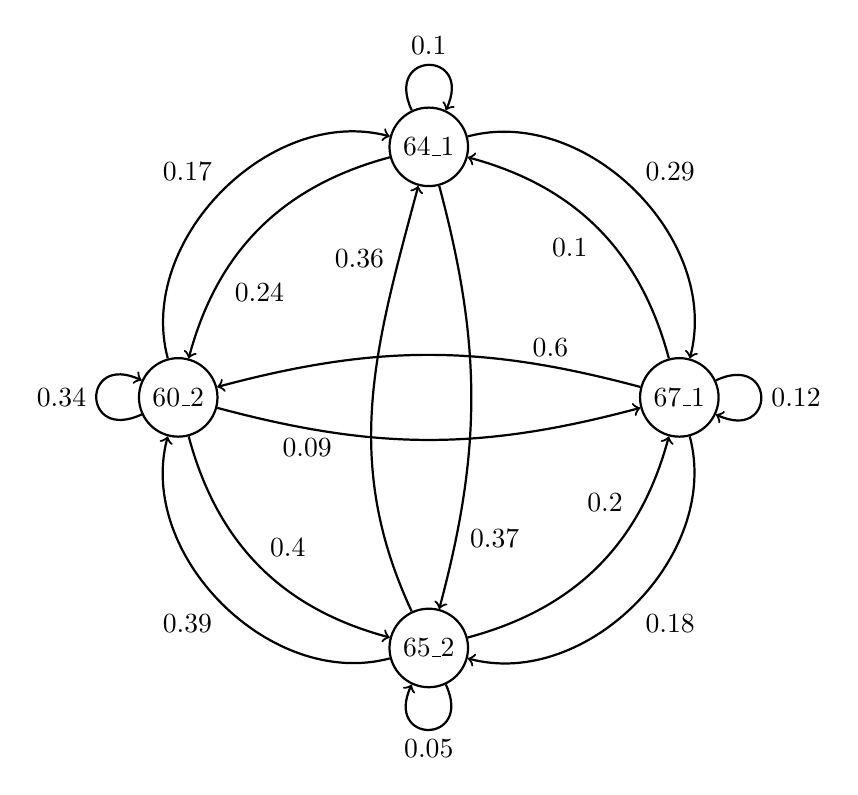
\begin{tikzpicture}[node distance={45mm}, thick, main/.style = {draw, circle}] 
    \node[main] (1) {$60\_2$}; 
    \node[main] (2) [above right of=1] {$64\_1$}; 
    \node[main] (3) [below right of=1] {$65\_2$};
    \node[main] (4) [below right of=2] {$67\_1$};
    \draw[->] (1) to [out=205,in=155,looseness=5] node[midway, left, pos=0.5] {0.34} (1);
    \draw[->] (1) to [out=105,in=165,looseness=1] node[midway, above left, pos=0.5] {0.17} (2);
    \draw[->] (1) to [out=-75,in=-195,looseness=1] node[midway, above right, pos=0.5] {0.4} (3);
    \draw[->] (1) to [out=-15,in=195,looseness=1] node[midway, below , pos=0.2] {0.09} (4);
    \draw[->] (2) to [out=195,in=75,looseness=1] node[midway, below right, pos=0.7] {0.24} (1);
    \draw[->] (2) to [out=115,in=65,looseness=5] node[midway, above, pos=0.5] {0.1} (2);
    \draw[->] (2) to [out=-75,in=75,looseness=1] node[midway, below right, pos=0.8] {0.37} (3);
    \draw[->] (2) to [out=15,in=75,looseness=1] node[midway, above right, pos=0.5] {0.29} (4);
    \draw[->] (3) to [out=195,in=255,looseness=1] node[midway, below left, pos=0.5] {0.39} (1);
    \draw[->] (3) to [out=115,in=255,looseness=1] node[midway, above left, pos=0.8] {0.36} (2);
    \draw[->] (3) to [out=295,in=245,looseness=5] node[midway, below, pos=0.5] {0.05} (3);
    \draw[->] (3) to [out=15,in=255,looseness=1] node[midway, above left, pos=0.7] {0.2} (4);
    \draw[->] (4) to [out=165,in=15,looseness=1] node[midway, above, pos=0.2] {0.6} (1);
    \draw[->] (4) to [out=105,in=-15,looseness=1] node[midway, below left, pos=0.5] {0.1} (2);
    \draw[->] (4) to [out=-75,in=-15,looseness=1] node[midway, below right, pos=0.5] {0.18} (3);
    \draw[->] (4) to [out=25,in=-25,looseness=5] node[midway, right, pos=0.5] {0.12} (4);
    \end{tikzpicture}
    \caption{Representación visual de la cadena obtenida a partir de la matriz de transición} 
    \label{fig:sampleNotesChain}
    \end{figure}

    \subsection{Generar melodías con Cadenas de Markov}
    \label{subsec:generarCadenasMarkov}
    Para crear melodías, podemos realizar el número de iteraciones que queramos sobre la cadena para crear una melodía de la longitud deseada, el acercamiento más simple sería generar N notas. 
    
    En nuestro generador (definido en el archivo \textit{MarkovGenerator.py}) se puede especificar el número de steps deseado y se generarán iteraciones suficientes hasta llegar al límite. Al ejecutar comenzamos siempre en "C4\_2", por conveniencia.

    \subsection{Puntos fuertes y débiles de la generación de melodías con Cadenas de Markov}
    \label{subsec:ventajasYDesventajasMarkov}
    Las cadenas de Markov resultan muy potentes como primer acercamiento, pues son un modelo simple y fácil de entender. El entrenamiento es sencillo y su ejecución una vez entrenada es prácticamente instantánea.

    Además, una parte importante es que al existir aleatoriedad es un modelo que no es determinista, por lo que cada ejecución será distinta.

    Sin embargo, tienen algunas desventajas:
    \begin{itemize}
        \item Primero, hablando de rendimiento y escalabilidad, cada nodo de la cadena tiene que representar una nota con duración como mínimo, por lo que en la práctica se crea una cadena inmensa aunque limitemos a 2 octavas el posible rango melódico. Esto hace que la cadena ocupe bastante en archivo, al menos con la librería que utilizamos.
        \item Desde el punto de vista musical, no proporcionan una melodía muy rica, ya que dependen completamente de la probabilística, las melodías generadas no tendrán una coherencia aparente. Aunque ese punto no resulta muy crítico para nuestro trabajo por el resto de etapas que realizamos, es conveniente obtener una melodía lo más agradable posible.
    \end{itemize}
    
    A pesar de las desventajas que presentan, son muy interesantes como modelo más experimental y liviano en la ejecución.

\section{Redes Neuronales Recurrentes}
\label{sec:RNR}
    \subsection{Introducción a las Redes Neuronales Recurrentes}
    \label{subsec:introRNR}

    \subsubsection{¿Qué es una red neuronal?}
    \label{subsub:introRedesNeuronales}
    Las redes neuronales son uno de los principales modelos de machine learning y de los más estudiados por su versatilidad y capacidad de resolver problemas no lineales. A lo largo de los años se han explorado muchos tipos de redes neuronales, pero antes de profundizar debemos de entender qué es una red neuronal. En esta sección se explicarán las redes neuronales de una forma muy simple y superficial para poder seguir el resto del trabajo, para más información sobre el tema y profundizar en sus bases es recomendable consultar \cite{M.A.Nielsen}.
    
    Las redes neuronales son, de forma simplista, una serie de nodos (llamados \textit{neuronas}) que contienen una función (llamada \textit{función de activación}). Los nodos se agrupan por capas y cada uno está conectado a todos los de la capa siguiente mediante unas conexiones llamadas \textit{pesos}. Esto implica que podemos representar una red de neuronas con un grafo como el de la Figura \ref{fig:simpleNN}.

    En toda red neuronal poseemos 3 tipos de capas principales: 
    
    \begin{itemize}
        \item Capa de entrada: codifica, como su nombre indica, la entrada de la red. La entrada de la red puede ser de muchos tipos dependiendo del problema, pero es típico adaptarla para que sea una serie de números reales, generalmente normalizados.
        \item Capa de salida: representa una codificación de la salida de la red. Al igual que la entrada, la salida de la red puede ser codificada de diversas maneras, siendo común la representación mediante \textit{one-hot encoding}.
        \item Capa oculta: puede ser una o varias dependiendo de la red. Esta capa se conecta a la entrada y la salida y actúa como intermediario de la red, permitiendo realizar el "aprendizaje". 
    \end{itemize}

    Las técnicas de codificacón más comunes incluyen: 
    \begin{itemize}
        \item Normalización de valores que son números enteros o reales: en este caso la entrada puede ser por ejemplo una distancia, la intensidad de un color, etc. Con la normalización conseguimos reducir la posible diferencia entre valores, lo que permite un mejor aprendizaje de la red.
        \item \textit{One-hot enconding}: este tipo de codificación resulta vital para poder codificar valores de tipo \textit{labeled}, es decir, valores discretos que se encuentran etiquetados, como por ejemplo un tipo de animal (perro, gato, koala, hurón...). El \textit{one-hot encoding} consiste en covertir estos valores en un array de tantos elementos como etiquetas existan y posteriormente rellenarlo con ceros en todos los elementos exceptuando el que se corresponda con la etiqueta a codificar, que tendrá valor 1.
    \end{itemize}

    El entrenamiento de una red consiste en dar valores a las conexiones entre neuronas (pesos) para que la salida sea la experada en cada caso. El proceso más común de entrenamiento es utilizar el \textit{stochastic gradient descent}, que consiste en realizar diversas iteraciones con subdivisiones de todos los datos de entrenamiento (llamadas batches). El \textit{stochastic gradient descent} irá minimizando el error de la salida hasta un punto de estancamiento.

    \begin{figure}
        \centering
        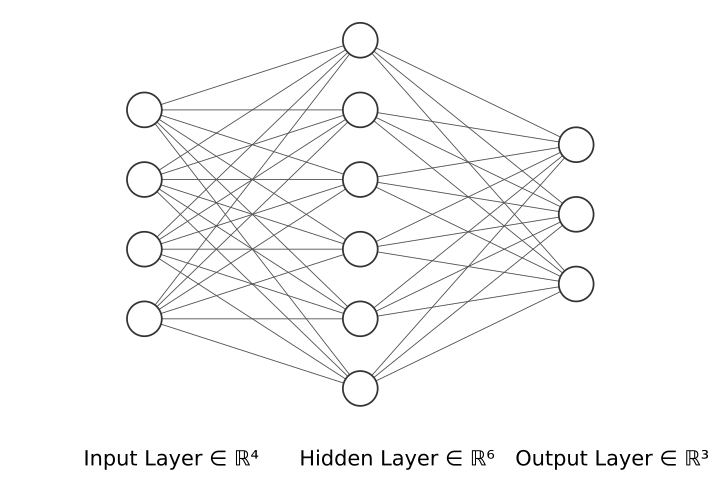
\includegraphics[width=1\textwidth]{Imagenes/Bitmap/nn.png}
        \caption{Red neuronal simple, con 1 capa oculta}
        \label{fig:simpleNN}
    \end{figure}

    \subsubsection{Introducir recurrencia a las redes}
    \label{subsub:introRedesNeuronalesRecurrentes}
    Una red neuronal clásica es buena realizando predicciones sobre una situación concreta o clasificando estados fijos, pero, ¿qué pasa si los datos que tenemos dependen de los que vinieron antes?

    Las redes neuronales recurrentes (RNN para abreviar) son redes neuronales en las que la salida se conecta a la entrada de la propia red, por lo que la salida en un instante depende de las salidas anteriores de la red.

    En estas redes podemos interpretar que la salida en un instante \textit{t} depende de la entrada en ese instante y de las salidas en los instantes \textit{t-1} y \textit{t-2} de la red, como se muestra en la Figura \ref{fig:simpleRNN}.

    \begin{figure}[h]
        \centering
        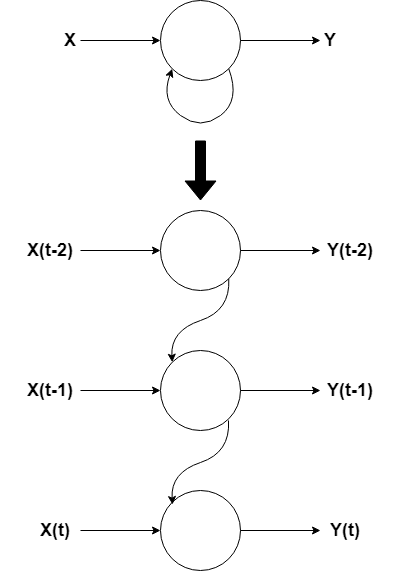
\includegraphics[width=0.5\textwidth]{Imagenes/Bitmap/RNN.png}
        \caption{Despliegue temporal de una RNN}
        \label{fig:simpleRNN}
    \end{figure}

    Las redes neuronales recurrentes son el modelo ideal para realizar predicciones de modelos financieros, modelos de reconocimiento y tratamiento de texto (conocido como NLP) y en nuestro caso, generar melodías que tienen en cuenta las notas anteriores de esta.

    Sin embargo, las RNN tienen un problema grave, al ser entrenadas utilizando el método del \textit{stochastic gradient descent} podemos apreciar el problema del \textit{desvanecimiento del gradiente} (consultar más información en \cite{M.A.Nielsen_Chapter5}). Este problema se encuentra en redes neuronales profundas de muchas capas y en redes recurrentes, pues al calcular el gradiente a lo largo de todas las capas este va disminuyendo, llegando a ser muy pequeño a medida que se llega a las primera capas de la red, esto hace que el entrenamiento se estanque y la red no consiga aprender correctamente. Este problema es instrínseco de estos tipos de redes, y es muy complicado evitarlo, para ello se utilizan modelos de redes neuronales recurrentes adaptados específicamente para reducir este problema.

    \subsubsection{Redes Long-Short Term Memory}
    \label{subsub:redesLSTM}
    Una forma de evitar el problema del \textit{desvanecimiento de gradiente} es utilizar el modelo Long-Short Term Memory, dicho modelo fue presentado en \cite{LSTMArticle}.

    La idea es introducir 2 vías de memoria a la red, uno de memoria a corto plazo y otro a largo plazo, la memoria a largo plazo se conecta a toda la red y la memoria a corto plazo se conecta a cada capa de la red. Combinando ambos tipos de memoria conseguimos que la red no desvanezca el gradiente. Consultar \cite{LSTMWikipedia} para más información.

    \subsection{Diseño de nuestra RNR}
    \label{subsec:disenoRNR}
    Para crear y entrenar nuesra red neuronal recurrente hemos utilizado la librería \textit{Keras}, propiedad de Google y que utiliza \textit{Tensorflow} como backend.

    La red tiene las siguientes capas:
    \begin{itemize}
        \item Capa input: una capa de entrada de 3 neuronas. La entrada consiste en el \textit{pitch} de la nota actual, la duración de la nota en \textit{steps} y el instante en el que suena la nota también en \textit{steps}.
        \item Capa LSTM: una capa, como su nombre indica, de tipo \textit{Long-Short Term Memory}. Esta capa hace el trabajo principal de la red, pudiendo procesar secuencias de notas para generar notas con un mayor contexto.
        \item Capa output: una capa de salida con 2 salidas independientes. Por un lado la nota predicha y por otro lado el \textit{start\_time} de dicha nota.
    \end{itemize}

    La entrada se normaliza antes de entrenar y se guardan los parámetros de normalización (la media y desviación típica) en un archivo JSON, para posteriormente poder normalizar la entrada cada vez que se ejecute. 

    Ya que utilizamos una capa LSTM, la entrada tiene que venir dada en forma de secuencias. En nuestra red, se utilizan secuencias de 5 como entrada, para las cuales se predice una salida.

    En el proceso de pruebas y mejoras del diseño de la red, se tomaron muchos enfoques. Una idea fue utilizar, como se dice anteriormente, una salida que prediga el tiempo de inicio de la nota, para introducir mayor dinamismo a la melodía. Sin embargo, dicho parámetro no aprendía correctamente patrones en el entrenamiento, aún utilizando una gran cantidad de datos, por lo que se decidió ignorarlo en la versión final. Aún así, para introducir silencios a la melodía se definen notas adicionales que representan silencios, lo cual producen mejores resultados que no tener silencios en toda la melodía.

    Finalmente, en la salida no se elige una nota arbitrariamente, sino que existe una serie de notas que han aparecido a lo largo del entrenamiento. La salida se encuentra codificada utilizando \textit{one-hot encoding} y representa la nota de tipo \textit{label} que predice la red que es la más adecuada. Este acercamiento nos permite utilizar una última capa de tipo \textit{softmax}, la cual permite añadir un factor aleatorio a la generación, ya que si no sería un modelo determinista y, por lo tanto, cada ejecución sería idéntica.
    
    \subsection{Resultados}
    \label{subsec:resultadosRNR}
    Con el uso de RNR conseguimos mejorar la calidad de las melodías que se generaban utilizando cadenas de Markov. Al introducir secuencias de notas, la red posee mayor contexto y puede realizar predicciones más acertadas, así como disminuir el factor aleatorio.

    Su ejecución resulta más cómoda, pudiendo variar la temperatura con la que generar para conseguir melodías más simples o más experimentales.

    Como aspectos negativos cabe destacar que su ejecución es más lenta, teniendo que calcular cada iteración individualmente, aunque no supone un problema grave de rendimiento.

    En definitiva, las redes neuronales recurrentes suponen un paso más en la calidad musical de las melodías, pero vamos a explorar modelos ya entrenados a continuación.

\section{Generación con Magenta}
\label{sec:magenta}
Tal y como se dijo en el estado de la cuestión, Magenta contiene una serie de modelos de \textit{machine learning} ya entrenados para disciplinas como la generación musical (ver Sección \ref{subsec:definicionMagenta}). Magenta posee varios paquetes que podemos utilizar para generar. A continuación se explican los diferentes paquetes y la integración en nuestra aplicación.

    \subsection{Paquete de Magenta para Python}
    \label{subsec:magentaPython}
    Existe un paquete de Magenta para Python, que puede ejecutar todos los modelos preentrenados.

    Dicho paquete tiene instrucciones de instalación para sistemas Linux y MacOS (consultar \cite{MagentaRepo}), sin embargo, a día de hoy no parece tener una versión compatible con Windows, por lo que no podemos utilizarlo en nuestra aplicación.

    \subsection{Paquete de Magenta para JavaScript}
    \label{subsec:magentaJS}
    Magenta tiene también una versión para JavaScript, que se ejecuta sobre TensorFlowJS. Dicha versión es análoga a la de Python y permite ejecutar los modelos preentrenados.

    Magenta Studio utiliza esta versión de Magenta, tanto para el plugin de Ableton como en la versión de escritorio, por lo que podemos utilizar esta versión para incluir Magenta en nuestro proyecto.

    \subsection{Magenta en nuestro proyecto}
    \label{subsec:magentaEnNuestroProyecto}
    Para poder comunicar nuestro proyecto de Python con Magenta utilizamos el módulo de Python \textit{subprocess}.

    Podemos tener diversos scripts de NodeJS que son ejecutados por un script Python y se comunican por los argumentos del proceso y la salida estándar de este en formato JSON. 

    Actualmente tenemos 2 scripts: 
    \begin{itemize}
        \item Uno dedicado a continuar melodías ya creadas (magentaContinue.js). El script utiliza \textit{MusicRNN} para continuar la melodía dada.
        \item Otro para generar melodías (magentaGenerator.js). Este script utiliza \textit{MusicRNN} para continuar una melodía de 1 nota (Do4) y así generar las melodías.
    \end{itemize}

    En la aplicación tenemos la posibilidad de generar melodías con Magenta, requiriendo una conexión a internet para descargar y ejecutar el modelo preentrenado.

    \subsection{Ventajas y desventajas de la generación con Magenta}
    \label{ventajasYDesventajasMagenta}
    Generar melodías con Magenta nos aporta varias ventajas:

    \begin{itemize}
        \item Son modelos entrenados con una gran cantidad de datasets y que utilizan técnicas avanzadas de \textit{machine learning}, por tanto, la generación de melodías es bastantes rica y estas poseen más coherencia interna.
        \item El \textit{continue} nos permite alargar melodías y mantenerlas coherentes para poder trabajar con ellas posteriormente.
    \end{itemize}

    Sin embargo, como desventaja principal tenemos la necesidad de una conexión a internet para poder utilizar el modelo, así como el tiempo que tarda el modelo en inicializar, sobre todo al tener que manejar subprocesos.

    Este modelo de generación nos aporta bastantes ventajas, pero es necesario mantener algún modelo que se pueda ejecutar de forma local y no dependa de módulos que a futuro puedan ser descontinuados.